%!TEX root = ../main.tex
\documentclass[../main.tex]{subfiles}
\begin{document}

  \chapter{Mathematics of Discretization}\label{chapter:fdes}
  The major benefit of studying equations which hold the form of a Transport equation is the large body of research of their solutions and behavior. We begin this chapter by considering the most basic transport equation, the Advection Equation which will allow the introduction of finite difference techniques.

  We then follow this through with a discussion of the approach used by \cite{hartvig2011} on the food web framework that they have developed using semi-implicit methods.

  \section{Advection Equation}
  The Advection Equation is a simple hyperbolic partial differential equation, in one dimension we take

  \begin{equation} \label{diff:eq:advection}
    \frac{\partial u}{\partial t} + v \frac{\partial u}{\partial x} = d u,
  \end{equation}

  for some transfer velocity $v$ and destruction rate $d$ on the domain $\mathbb{R}^+ \times R$ for some $R \subseteq \mathbb{R}$. The linear advection has been studied extensively and thus we can gain some insight in to potential issues that might occur in our more complicated equations such as \autoref{model:eq:logscale}.

  \subsection{Analytic Solution}
  As with ordinary differential equations, partial differential equations can be solved with the ``method of characteristics'' (or method of lines). Say we consider \autoref{diff:eq:advection} on the domain $\mathbb{R}^+ \times \mathbb{R}^+$, as to line up with the McKendrick-von Foerster Equation. Then we define some boundary value and initial value problem (BVP and IVP):

  \begin{eqnarray} \label{diff:eq:advectionbvp}
    u_t + v \, u_x  &=& + d \, u \nonumber \\
    u(0, x) &=& I(x) \nonumber \\
    u(t, 0) &=& B(t)
  \end{eqnarray}

  Using the method of characteristics we consider a point in the domain $\{(t, x) : t, x > 0 \}$ and solve the equation along some characteristic line $(t(s), x(s)) = y(s)$ stemming from an $y_0 \in \Gamma = \{ (0, x) : x \in \mathbb{R}^+ \} \cup \{ (t, 0) : t \in \mathbb{R}^+ \}$. The full details of the method are left to the reader, or in Chapter 4 of \cite{holmes2006}, however we find that

  \begin{equation} \label{diff:eq:advectionsol}
    u(t, x) = \left\lbrace \begin{array}{ll}
      I(x - v t) \e{-d \, t} & x - vt > 0 \\
      B(x - v t) \e{-d \, t} & x - vt \leq 0 \\
  \end{array} \right.
  \end{equation}

  along any characteristic $x = vt$. We note that the McKendrick-von Foerster equation will take a form similar to this if the growth and death terms are constants, but the problem will become more complicated if the coefficients are functions of $t, x$ or non-linear. However this problem does allow us to introduce the idea of \emph{domain of dependence}.

  Given any BVP and/or IVP on $U \subseteq \mathbb{R}^n$ the with solution $\varphi$, the domain of dependence for for any $x \in U$ is the set $V \subseteq U$ that $\varphi(x)$ depends on to be calculated. \autoref{diff:fig:domainofdep} shows the characteristic lines for, the blue lines represent characteristics which depend on the time axis boundary condition while the red arrows depend on the spatial axis initial condition. Looking at the analytic solution to \autoref{diff:eq:advectionbvp} we see that the initial condition is carried along the characteristic.

  \begin{figure}[htb]
    \centering
    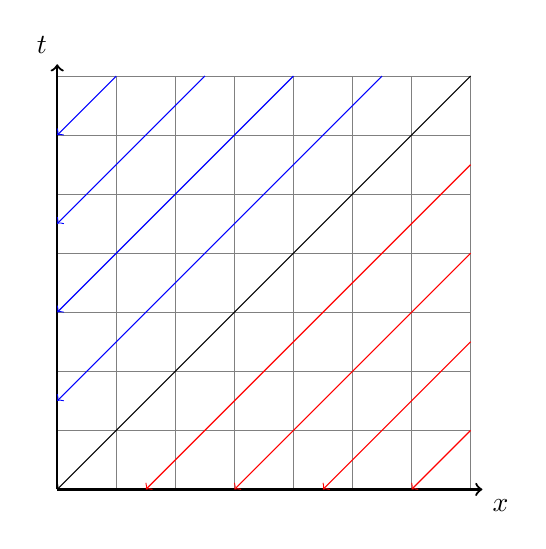
\begin{tikzpicture}[scale=0.75]
      \draw[help lines] (0,0) grid (7,7);

      \draw[thick, ->] (0, 0) -- (0, 7.2) node[anchor=south east] {$t$};
      \draw[thick, ->] (0, 0) -- (7.2, 0) node[anchor=north west] {$x$};

      \draw[blue, <-] (0, 1.5) -- (5.5, 7);
      \draw[blue, <-] (0, 3) -- (4, 7);
      \draw[blue, <-] (0, 4.5) -- (2.5, 7);
      \draw[blue, <-] (0, 6) -- (1, 7);

      \draw[<-] (0, 0) -- (7, 7);

      \draw[red, <-] (1.5, 0) -- (7, 5.5);
      \draw[red, <-] (3, 0) -- (7, 4);
      \draw[red, <-] (4.5, 0) -- (7, 2.5);
      \draw[red, <-] (6, 0) -- (7, 1);
    \end{tikzpicture}

    \caption{The characteristic lines for the solution of \autoref{diff:eq:advectionsol} with constant coefficients. There is no overlap between the lines which means that the solution can be smooth if the boundary conditions along $\Gamma$ are smooth. The domain of dependence for traverses the direction of each arrowhead line. \label{diff:fig:domainofdep}}
  \end{figure}

  While it is not obvious how this definition will be useful now, it will become extremely important in the analysis of stability of the numerical methods that we discuss in the next chapter.

  \subsection{Numerical Solutions to the Advection Equation} \label{diff:sec:fdesintro}
  Suppose now that we want to solve the advection numerically. Writing the equation using limits we have that

  \begin{equation} \label{diff:eq:finiteadvection}
    \lim_{\Delta t \to 0} \frac{u(t + \Delta t, x) - u(t, x)}{\Delta t} + v \lim_{\Delta x \to 0} \frac{u(t, x + \Delta x) - u(t, x)}{\Delta t} = d u(t, x).
  \end{equation}

  However what if we simply ignored the limits and used Newtonian infinitesimals $\Delta t, \Delta x$? This would give us the equation

  \begin{equation} \label{diff:eq:advectionfde}
    \frac{u(t + \Delta t, x) - u(t, x)}{\Delta t} + v \frac{u(t, x + \Delta x) - u(t, x)}{\Delta x} = d u(t, x)
  \end{equation}

  which can be rearranged to solve for $u(t + \Delta t, x)$. This would give a discrete way of calculating a next time step  of the solution to the equation ($u(t + \Delta t, R)$) if we knew the solution $u(t, R)$. This forms the fundamental idea for finite difference equations. These equations approximate a problem by considering a discrete mesh on the domain and then solving the equation using a consistent (see \autoref{diff:sec:consistency}) difference equations.

  \section{Difference Equations}
  In general, most partial differential equations do not have explicit analytic solutions. Consequently we must find accurate numerical approximations and methods for solving these problems. In this section we introduce the required mathematics for understanding the numerical methods used to solve problems in partial differential equation theory.

  \cite{boole1880} writes \emph{``Differential Calculus is occupied about the limits to which such ratios approach as the increments are indefinitely diminished.'' However, ``The Calculus of Finite Differences may be strictly defined as the science which is occupied about the ratios of the simultaneous increments of quantities mutually dependent.''} In simple terms the calculus of finite differences is only concerned about ratios of infinitesimals, in line with the ideas of Newtonian calculus.

  In \autoref{diff:eq:finiteadvection} we broke down the limits in the derivitives by simply ignoring the limit, in this section we reconstruct this equation using difference equations derived from \cite{boole1880} and \cite{hildebrand1987}.

  \begin{definition}[First Forward Difference]
    For a function $u: U \to \mathbb{R}$ the first forwards difference of $u$ is

    \begin{equation}
      \Delta_f[u](x) = u(x + \delta x) - u(x).
    \end{equation}
  \end{definition}

  \begin{definition}[First Backwards Difference]
    For a function $u: U \to \mathbb{R}$ the first backwards difference of $u$ is

    \begin{equation}
      \Delta_b[u](x) = u(x) - u(x - \delta x).
    \end{equation}
  \end{definition}

  These two definitions form the basis for finite difference theory, and we can take any difference $\Delta[u](x)$ as a combination of forward and backward differences. Just as with the differential operator we have that the difference operator is linear and satisfies the Leibniz rule. The proof of this is left to the reader, but follows exactly the same method as for derivatives. It is easy to construct the $n^{th}$ difference ($\Delta ^n[f](x)$) by simply considering $\Delta [\Delta ^{n-1}[f]](x)$.

  When we consider the partial derivative of $u: \mathbb{R} \to \mathbb{R}$ we simply have that

  \begin{equation}
    u'(x) = \lim_{\delta x \to 0} \frac{\Delta[u](x)}{\delta x}
  \end{equation}

  which can easily be extended to higher dimensions.

  \subsection{Taylor's Theorem,  Big \& little O Notation}
  When calculating an equation we can replace terms by their approximate sizes if, for instance, the exact size is not required. In such cases we generally replace terms by their big (or little) O size. If $f, g : \mathbb{R} \to \mathbb{R}$, the informal assertions that $f(x)$ is big-O (or little-O) of $g(x)$ can be rigorously defined by comparing their sizes in limits around a point.

  \begin{definition}[Big O]
    We formally define that
    \begin{equation}
      f(x) = O(g(x))
    \end{equation}
    as $x \to a$ if and only if
    \begin{equation}
      \limsup_{x \to a} \left\vert \frac{f(x)}{g(x)} \right\vert < \infty
    \end{equation}
  \end{definition}

  \begin{definition}[Little O]
    We define
    \begin{equation}
      f(x) = o(g(x))
    \end{equation}
    as $x \to a$ if
    \begin{equation}
      \lim_{x \to a} \left\vert \frac{f(x)}{g(x)} \right\vert = 0
    \end{equation}
  \end{definition}

  Intuitively calling $f(x)$ big-O of $g(x)$ states that $f(x)$ is ``about as big'' as $g(x)$, while if $f(x)$ is little-o of $g(x)$ then it is ``much smaller'' in size that $g(x)$. A very classical theorem in calculus is Taylor's theorem, which finite difference

  \begin{theorem}[Taylor]
    If $u : \mathbb{R} \to \mathbb{R}$ is $k$ times differentiable in a region around $x \in \mathbb{R}$ then $u(x + \delta x)$ can be written as

    \begin{equation} \label{diff:eq:taylor}
      u(x + \delta x) = u(x) + (\delta x) \, u'(x) + ... + \frac{(\delta x)^k}{k!} u^{(k)}(x) + h_k(x + \delta x) (\delta x)^k
    \end{equation}

    for some function $h_k(x)$ such that $\lim_{\delta x \to 0} h_k(x + \delta x) = 0$.
  \end{theorem}

  If \autoref{diff:eq:taylor} is reformulated to give a polynomial estimation $P(x)$ for $u(x)$ then the approximation error for a taylor polynomial $R_k(x) = u(x) - P_k(x)$ can be estimated as $o((\delta x)^k)$. Using this theorem we know that if $u$ is a differentiable function then by taking $k = 1$ that

  \begin{equation}
    u(x + \delta x) = u(x) + \delta x u'(x) + o(\delta x)
  \end{equation}

  and so we can take the difference equation

  \begin{equation} \label{diff:eq:bigoapprox}
    \frac{\Delta[u](x)}{\delta x} = u(x) + O(\delta x)
  \end{equation}

  an approximation to a first derivative of $u$. Given a difference equation $d_k(x)$ that depends on $k = \delta x$ that represents the left hand side of \autoref{diff:eq:bigoapprox} that approximates an $n^{th}$ derivative of $u$ we define the order of the approximation to be the integer $N$ that satisfies

  \begin{equation}
    d_k(x) - u^{(n)}(x) = O(k^N).
  \end{equation}

  \section{Finite Difference Equation Errors}
  Since finite difference equations have become such a staple in numerical analysis there are many texts that supply the different coefficients required to approximate derivatives accurately. By combining $n^{th}$ forward and backward differences we can construct higher order approximations to derivatives at higher orders and higher orders of accuracy and \cite{fornberg1988} provides a details derivation, as well as, a set of tables for almost all derivatives required for general PDE problems up to high orders in both accuracy and order. We define a \emph{finite difference scheme} as a particular choice of approximation for a collection of derivatives.

  However as with all numerical problems issues arise when constructing approximations due to errors that occur with the generation of those approximations themselves. In this section we begin to outline the two main types of error that occur in approximations and introduce the idea of consistency and convergence.

  \subsection{Notation}
  Before we move forward discussing the rigorous theory of finite difference equations, their errors and use to approximate partial differential equations we introduce some general theory. As we have seen in \autoref{chapter:sizetheory} we will deal with equations with the form

  \begin{equation} \label{diff:eq:pdeprob}
    L(u) = \frac{\partial u(t, x)}{\partial t} - \mathcal{L}(u(t, x)),
  \end{equation}

  where $\mathcal{L}$ is a $m$ times differential operator in $x$ (with most cases satisfying $m < 3$). Given this we have that if $u$ is in the set of real valued functions, $C^m$, which are a one times differentiable function in $t$ and $m$ times differentiable function in $x$ on some region in the plane $\Omega = \mathbb{R}^+ \times U$ for some $U \subset \mathbb{R}^+$ then $L : C^M \to C$. We aim to solve the partial differential equation $L(u) = 0$ with boundary conditions the boundary of $\Omega$.

  To do this we first discretise our domain in to a mesh grid. In \autoref{diff:fig:meshgrid} we discretise an area of the plane $[0, T] \times [0, X]$ in to a grid spaced with $\delta x = k$ and $\delta t = h$. We index the time axis by $n$ and the spatial axis by $j$, thus for any function $u : [0, T] \times [0, X] \to \mathbb{R}$ we write $u(t, x) = u(n h, j k) = u^n_j$.

  \begin{figure}[hbt]
    \centering
    \begin{tikzpicture}
      \draw[help lines] (0, 0) grid (6, 6);

      \draw[thick, ->] (0, 0) -- (0, 7.2) node[anchor=south east] {$t$};
      \draw[thick, ->] (0, 0) -- (7.2, 0) node[anchor=north west] {$x$};
      \draw (0, 0) -- (6, 0) -- (6, 6) -- (0, 6);
      \node[anchor=east] (t) at (0, 6) {$T$};
      \node[anchor=north] (t) at (0, 6) {$X$};

      \draw[fill=black] (3, 3) circle (0.1cm);
      \node[anchor=north west] (name) at (3, 3) {$u^n_j$};

      \node[anchor=east] (j) at (0, 4) {$n+1$};
      \node[anchor=east] (j) at (0, 3) {$n$};
      \node[anchor=east] (j) at (0, 2) {$n-1$};

      \node[anchor=north] (n) at (4, 0) {$j+1$};
      \node[anchor=north] (n) at (3, 0) {$j$};
      \node[anchor=north] (n) at (2, 0) {$j-1$};

      \draw[thick, <->] (2, -0.7) -- (3, -0.7) node[anchor=north east] {$k$};
      \draw[thick, <->] (-1.2, 2) -- (-1.2, 3) node[anchor=north east] {$h$};
    \end{tikzpicture}

    \caption{An example mesh-grid for the region $[0, T] \times [0, X]$ with an illustration of a grid on the central region of the domain. \label{diff:fig:meshgrid}}
  \end{figure}

  With this numerical realization of the domain for a partial differential equation, and a choice of finite difference scheme we construct a finite difference equation $D^n_j$ which takes a $C^m$ function, $u$, and returns a combination of $u^m_i$ for relative values of $m$ and $i$ to $n$ and $j$.

  \begin{example}
    Consider the advection equation again with a first order approximation for the time and spatial derivatives. Then our finite difference equation states that

    \begin{equation} \label{diff:eq:advectionexample}
      D^n_j(u) = \frac{1}{h} u^{n+1}_j + \left( \frac{\upsilon}{k} \right) u^n_{j+1} + \left( \frac{-1}{h} - \frac{\upsilon}{k} \right) u^n_j.
    \end{equation}
  \end{example}

  \subsection{Consistency} \label{diff:sec:consistency}
  When considering the appropriateness of a finite difference equation to model a particular problem there are three problems that arise, the most easy of these to understand is consistency. The broad definition of consistency is that a finite difference equation $D$ is consistent with a partial differential equation $L$ if the truncation error of $D$ from $L$ tends to $0$ for smaller mesh grid approximations.

  To formally introduce consistency consider a PDE in them form of \autoref{diff:eq:pdeprob} with a true solution $\Phi$. Suppose that we take any finite difference equation $D^n_j$ to approximate \autoref{diff:eq:pdeprob} and let $\phi$ be a non-zero solution to $D(u) = 0$.

  \begin{definition}[Truncation Error]
    For any problem described above the \emph{Truncation error} for a function $\psi : \Omega \to \mathbb{R}$ at any grid point $(n, j)$ is given as

    \begin{equation}
      T^n_j(\psi) = D^n_j(\psi) - L^n_j(\psi)
    \end{equation}

    where $L^n_j$ represents $L(u)$ evaluated at $(t, x) = (n h, j k)$.
  \end{definition}

  % Clear up global truncation error
  While we can consider the global truncation of a finite difference approximation, by considering $D$ acting upon arbitrary functions $v$, if $v = \Phi$ is the true solution of $L$ and is known then the local truncation error $\tau^n_j$ is defined as $T^n_j(\Phi)$. If $\tau^n_j = O(h^p)$ then $Dv$ is said to be an approximation order $p$ method, and in reality most finite difference equations are of order $p$ for some $p \in \mathbb{N}$. However this is not always the case and this is why we rely on consistency in a numerical calculation. $T^n_j$ gives an estimate of the error of replacing $L^n_j(v)$ by $D^n_j(v)$. This gives arise to a formal definition of consistency.

  \begin{definition}[Consistency]
    A finite difference approximation $D^n_j$ is consistent to a partial differential equation $L$ as described above. Then if $v$ is any function, with a sufficient number of continuous derivatives such that $L^n_j(v)$ can be evaluated, $D^n_j$ is considered consistent with $L$ if

    \begin{equation}
      \lim_{k, h \to 0} T^n_j(v) = \lim_{k, h \to 0} D^n_j(v) - L^n_j(v) = 0.
    \end{equation}
  \end{definition}

  If $v = \Phi$ then $T^n_j(v) = \tau^n_j$, so another definition of consistency is that the limiting value of the local truncation error is $0$. Suppose that we review \autoref{diff:eq:advectionfde} as an approximation to \autoref{diff:eq:advection}, having engineered the scheme using \cite{fornberg1988} seen in \autoref{diff:eq:advectionexample} we know that rearranging to gain an equation in the form $D(u) = 0$ the truncation error can be written as

  \begin{equation}
    T(v) = D(v) - L(v) = O(h) + v O(k) - d O(1) = O(h) + O(k)
  \end{equation}

  and thus as $h, k \to 0$ then $T(v) \to 0$ and we have a consistent difference equation of order $p = 1$.

  \subsection{Stability}
  Numerical stability theory stems more directly from analytical stability theory. Suppose that $L(u)$ is a PDE problem with two analytic solutions $\Psi_1$ and $\Psi_2$, one can analyze how likely a perturbation in the initial condition is to affect the system as it tends to one of the two analytic solutions. This same principle applies to numerical methods. The essential idea defining stability is that the numerical process should not cause any small perturbations introduced through rounding at any stage to grow and ultimately dominate the solution, similar to the study of whether a small perturbation introduced into an analytic solution will cause the solution to tend to a dominant solution.

  For mathematical analysis a definition of stability is given with relation to the growth of the exact solution to the finite difference equation. Therefore if rounding errors of perturbations to the solution are introduced at any stage in time then these will also be bounded if the exact solution is bounded.

  \begin{definition}[Numerical Stability]
    A numerical method is stable if, for a fixed spatial domain $[0, X]$, for every $T > 0$ there exists a constant $c(T) > 0$ such that

    \begin{equation}
      || \boldsymbol\phi^n ||_k < c(T)
    \end{equation}

    for all $n = 0, 1, .. , T / h$ and $h \to 0$, $k \to 0$.
  \end{definition}

  The norm $|| \cdot ||_k$ is a grid dependent norm of , for example

  The norm $|| \cdot ||_k$ is a grid dependent Euclidean Norm for the space, for example

  $$
    || \mathbf{u} ||_k = \left( k \sum |u_j|^2 \right)^{1/2},
  $$

  acting on the vector $\boldsymbol\phi^n = (\phi^n_j : j = 0, .. , X / k) \in \mathbb{R}^{(X / k) + 1}$.

  \subsubsection{Eigenvalue Method}
  If a finite difference approximation can be written in matrix form $u^{n+1} = S^{n+1} u^0$, where $u^n$ represents a vector of the values of $u^n_j$ for all $j$ and $S^{n+1}$ is an invertible matrix which consolidates our finite difference approximation in to a matrix. Then we can determine the stability of that approximation by considering the eigenvalues of the matrix $S$. If all the eigenvalues, $\lambda_S$, of $S$ satisfy $| \lambda_S | \leq 1$ then we have that

  \begin{equation}
    |S^n z | < \infty
  \end{equation}

  as $n \to \infty$ for all vectors $z$. Thus, if we consider the eigenvalues for this matrix we can determine the stability of the system.

  \begin{example}
    Suppose that we consider the approximation for the advection equation see in \autoref{diff:eq:advectionexample}. This can be written in with $S$ in the tridiagonal form

    \begin{equation}
      \begin{pmatrix}
        a & b & \\
        c & a & b \\
          & c & \ddots & \ddots & \\
          &   & \ddots & a & b \\
          &   &        & c & a
      \end{pmatrix}
    \end{equation}

    and thus has eigenvalues $\lambda_j = a + 2 \sqrt{bc} \cos{\left( \frac{j \pi}{J} \right)}$ for $j = 1, ... , J-1$ if there are $J$ points in our mesh grid along the $x$ axis. Considering the worst case for this eigenvalue spectrum will yield a relation between $h$ and $k$ that must be satisfied for the method to be stable.
  \end{example}

  This way of analyzing the stability of a scheme is not easily generalized since it involves finding the eigenvalues of the corresponding S-matrix. Therefore we look at a different way of determining stability - the Fourier method or von Neumann method.


  \subsubsection{Fourier Method}
  The Fourier method is one of the most common methods for analyzing the stability of a finite difference equation. If the spatial differential operator, $\mathcal{L}$, in $L$ is linear then in the limit as $h, k \to 0$ the numerical error for a finite difference equation also satisfies $L$ since

  $$
    L(\phi - \Phi) = (\phi - \Phi)_t - \mathcal{L}(\phi - \Phi) = (\phi_t - \mathcal{L}(\phi)) - (\Phi_t - \mathcal{L}(\Phi)).
  $$

  We assume that the scheme admits a solution in the form

  \begin{equation}
    \upsilon^n_j = \lambda^n(\omega) \e{i j \omega \Delta x}
  \end{equation}

  and define

  \begin{equation}
    G(\omega) = \frac{\lambda^{n+1}(\omega)}{\lambda^n(\omega)}
  \end{equation}

  to give the amplification factor which governs the growth of the solution at each time step. The von Neumann stability condition is given by

  \begin{equation}
    \left\vert G(w) \right\vert \leq 1
  \end{equation}

  for all $0 \leq \omega \Delta x \leq \pi$. If a finite difference equation is stable then it is said to be conditionally stable if there is dependence on $G(\omega)$ for the stability condition to hold, otherwise the scheme is unconditionally stable. The Fourier method is the most widely used but can break down for non-linear methods since it can be more difficult to solve for $G(\omega)$.

  \section{Convergence Theory}
  In the previous section we defined the Truncation Error of a finite difference equation as the approximation error for a partial differential equation. In this section we deal with the numerical error.

  \begin{definition}[Numerical Error]
    Given a BVP/IVP problem with true solution $\Phi(t, x)$ and a finite difference equation $D(u)$ with true solution $\phi$ the numerical error of $\phi$ is defined as

    \begin{equation}
      e^n_j(u) = \phi^n_j - \Phi^n_j.
    \end{equation}
  \end{definition}

  Broadly speaking, we define convergence of a problem in a very simple way. Does our numerical solution accurately model the real solution. However the numerical error and true solution, and thus convergence, of a general problem is quite difficult to calculate since it relies on the knowledge of the solution. Thus we will need some more theory to deal with this issue. Before we move on to this theory we give the rigorous definition of convergence.

  \begin{definition}[Convergence]
    Given a BVP/IVP problem with true solution $\Phi(t, x)$ and a finite difference equation $D(u)$, with $\Delta t = h$ and $\Delta x = k$. The solution $D$, $\phi$, is said to converge to $\Phi$ if

    \begin{equation}
      \lim_{k \to 0} \left( \max_{n = 0, 1, ..., T / k} || \boldsymbol\phi_j - \boldsymbol\Phi_j ||_k \right) = 0.
    \end{equation}

    for every initial condition and for every $T > 0$
  \end{definition}

  The most major result in the theory of \emph{linear} finite difference equations is the  Lax–Richtmyer Equivalence theorem.

  \begin{theorem}[Lax-Richtmyer]\label{diff:theorem:lax}
    For a uniformly solvable linear finite difference scheme which is consistent with a well-posed linear evolution problem, the stability is a necessary and sufficient condition for its convergence.
  \end{theorem}

  In plain terms the theorem states that \textbf{Consistency + Stability implies convergence}. An extremely useful result which allows numerical mathematicians to ignore issues with finding the true solution of a PDE to calculate the convergence of finite difference equations.

  However the issues arises that this theorem only holds for \emph{linear} problems. Thus in our research on \autoref{model:eq:logscale} with non-linear coefficients the theorem will break down. Luckily \autoref{diff:theorem:lax} has been extended by the work of \cite{rosinger2008} who classes a more general set of partial differential equations using nonlinear semigroup theory.

\end{document}
